\chapter{Data sources} %TODO rename

\section{OpenStreetMap}

OpenStreetMap (OSM) is a collaborative community project to create a full, editable representation of our world. The project was founded in 2004 by Steve Coast, and now boasts over ten million registered volunteer users providing data from around the globe. Unlike proprietary services (such as Google Maps or Apple Maps), OSM data is open and freely available to build on or modify.\cite{osmHistory}

\subsection{Why OpenStreetMap?}

As my intentions with this thesis project included following free and open source software guidelines\ref{licensing}, OSM was a perfect match to allow for further potential derivate works. Its widespread use also makes it easy to find and import arbitrary cities' datasets into the program, practically removing the limit on the area covered.

The sheer amount of data stored on the platform can be difficult to work with; strong inferences can be made on anything from building height trends to bus route frequencies. This is mostly thanks to easy to use uploading tools, such as the web editor iD or the mobile app StreetComplete (see~\ref{scee}).

\begin{figure}[h]
    \centering
    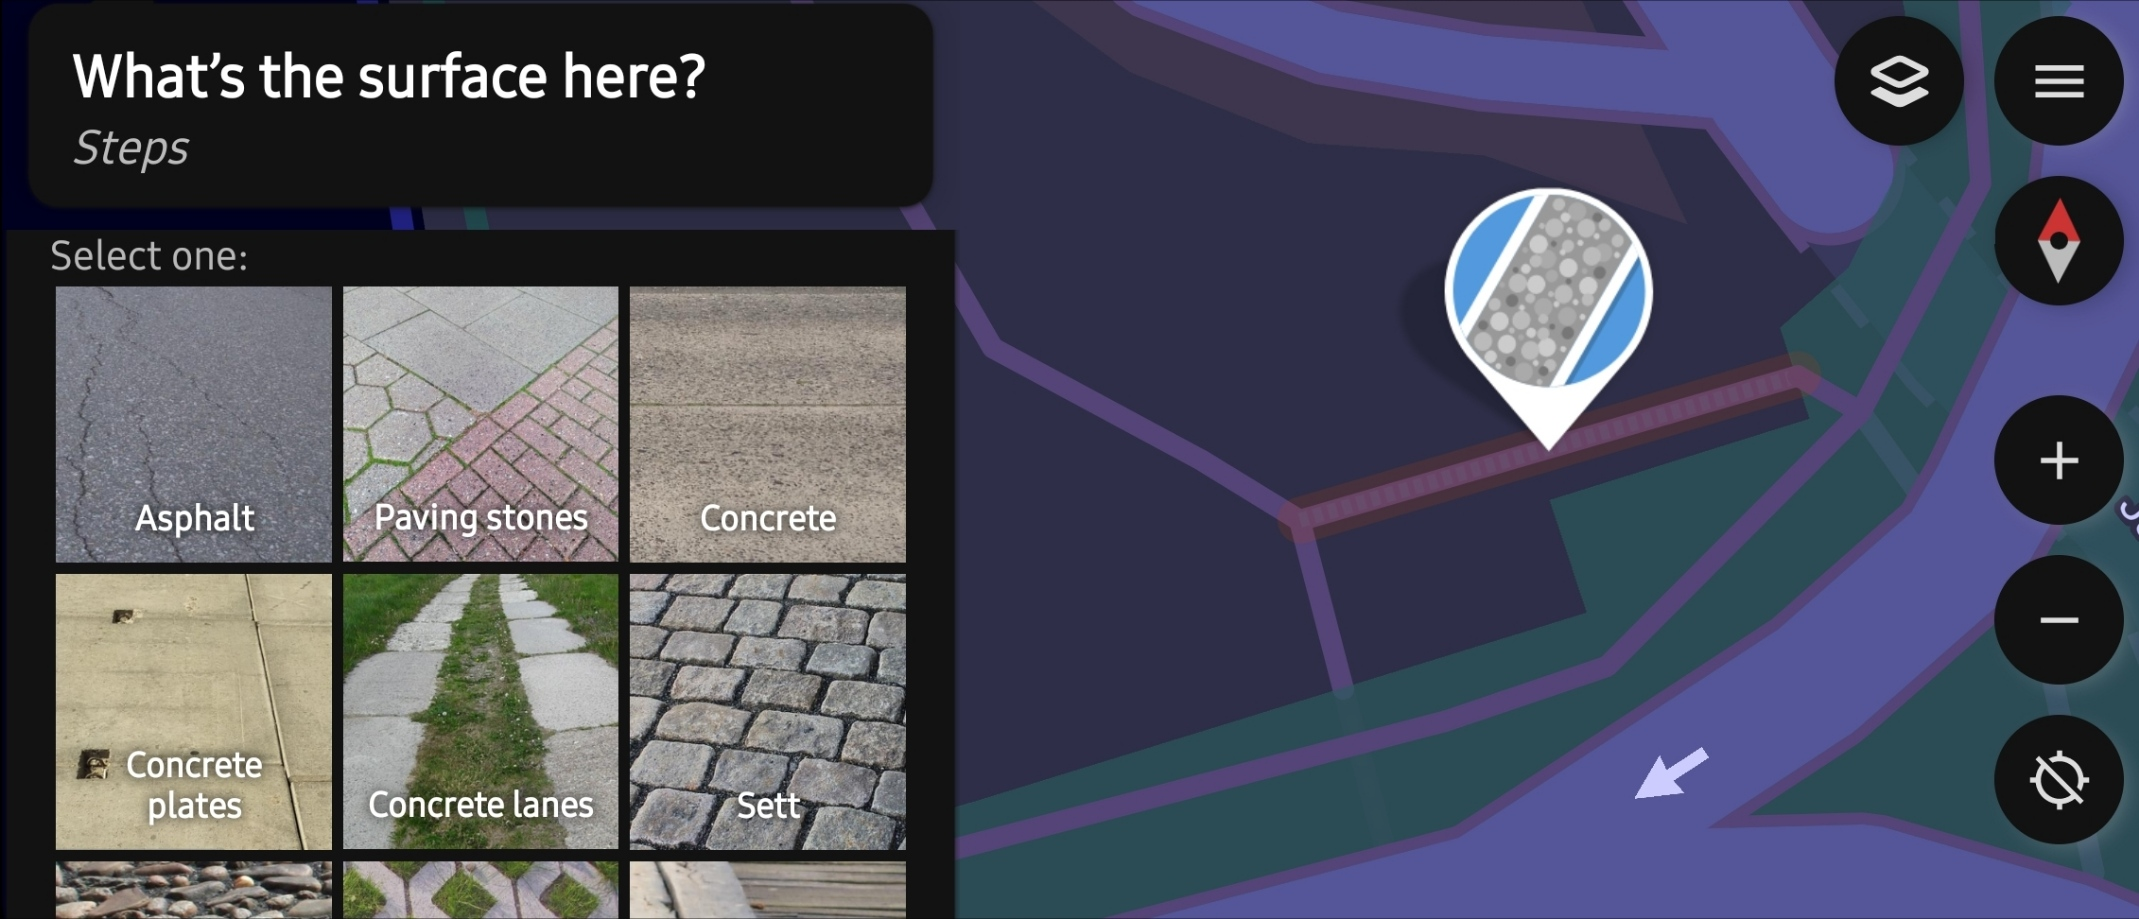
\includegraphics[width=140mm, keepaspectratio]{images/scee_example.jpg}
    \caption{A "quest" in the SCEE app, an improved version of StreetComplete; the user can submit information they see in real life \label{scee}}
\end{figure}

I also took a liking to discovering the mapping service powering most apps I use, and was interested in contributions to the dataset myself. Using it for my application would help me understand the inner workings better.

\subsection{Semantic data structure}

OpenStreetMap data is made up of elements -- nodes, ways and relations -- each describing some specific feature in space. Every element can contain multiple tags.~\cite{osmElements} Tags are simple key-value pairs which can store strings only, but may be used to represent complicated concepts. The meaning of each key is somewhat loosely defined and isn't standardised as there are over 96.000 of them -- guidelines do exist, however\footnote{\url{https://wiki.openstreetmap.org/wiki/Map_features}}. Using examples, they can range from \verb|name=Tüskesátor|, defining a simple building name, to \verb|source:maxspeed=HU:zone:30|, which details speed restrictions as applicable to a given road.

The simplest element is a node. They represent objects that can not or should not be described with as a complicated surface. For instance, a bench or newsstand would be difficult to represent as anything other than a point. Over nine billion of these nodes exist, with 64-bit integer identification numbers and seven decimal places of precision for their latitude and longitude. Declaring elevation above sea level is optional.

A way can combine multiple nodes into a polyline, a connected chain of points. This may be used to add a building outline or a road. The accuracy can depend on the author, as there is no curve interpolation; the more sparse the contained nodes are, the more jagged the way becomes. Over a billion ways exist, and they may be open (the last and first point is not connected) or closed. Buildings usually fall into the latter category.

Relations are catch-all elements and may represent anything more complex than a single way -- in fact, they're lists of nodes and ways with metadata added through tags. A complicated building may be treated as a relation, just as an intercity bus route is a connection of highways and streets. Child elements can have roles: for example, outer and inner building walls, or the main and side streams of a river.

\subsection{Technical data structure}

Live online data is most easily queried throught the Overpass API\footnote{\url{https://wiki.openstreetmap.org/wiki/Overpass_API}}. It provides read-only access to OSM elements and accepts a wide variety of filters. The returned information is JSON-convertible, making it ideal for apps that require more control than what pre-made webmap plugins can provide. Queries use a custom language that simplifies searching by key and supports recursion well. The Overpass Turbo\footnote{\url{https://overpass-turbo.eu}} app has a wizard that aids the creation of Overpass requests.

Data may also be distributed in a heavily compressed Protocolbuffer Binary Format (PBF\footnote{\url{https://wiki.openstreetmap.org/wiki/PBF_Format}}) file. BBBike\footnote{\url{https://download.bbbike.org/osm}} provides exports of many large cities, as well as the ability to download a file containing information on a zone up to 6000 by 4000 kilometers large. On the scale of the entire planet, PBF saves over 96\% of space usage when compared to regular XML. PBF files utilise Google's Protocol Buffer\footnote{\url{https://github.com/protocolbuffers/protobuf}} interchange format. Based on a schema specification (not unlike one made for databases), a protocol buffer compiler can create low-level, efficient code for serialisation into said schema. Each .pbf file is a series of binary blobs and their headers, ultimately encoding key-value pairs in a string format. The obvious downside is that reading this data now requires specialised libraries or custom classes that can decode and uncompress it. I depended on osm4j\footnote{\url{https://github.com/topobyte/osm4j}} for this task, as it has a simple iterator to unpack elements sequentially.
It's worth noting that PBF files store elements in the order of Node, Way, Relation. Relations and ways use foreign keys with a number format to connect to their child nodes. Earlier reads should thus be cached for later reference, only throwing away unneeded nodes as it becomes clear they're not part of any required relation -- this is analogous to how a garbage collector works.


\subsection{Examples and Visualizations}
